% AI-translated from the accepted LaTeX transcription of printed pp. 202--211, including unnumbered [205].
\begingroup
\clearpage
\noindent202\hfill\textsc{Remarks.}\hfill\mbox{}\par\medskip
\begingroup\footnotesize
\[
\begin{array}{r@{\qquad}l}
2)&\displaystyle \tfrac1{12}\frac{(1-ee\sin\varphi^2)^3}{a^4(1-ee)^3}
\{1-3ee+(ee+15e^4)\sin\varphi^2-14e^4\sin\varphi^4\}=\beta,
\end{array}
\]
then by Art.~[7], p.~154, we have
\[
\log n=\alpha yy-\beta y^4+\cdots.
\]
Let $x$ be positive southward, so that
\[
\begin{array}{r@{\qquad}l}
3)&\displaystyle\frac{\partial\alpha}{\partial x}
=\frac{\partial\alpha}{\partial\varphi}.\frac{\mathrm d\varphi}{\mathrm dx}
=+\frac{ee\sin2\varphi(1-ee\sin\varphi^2)^{\frac52}}{a^3(1-ee)^2}=\gamma
\end{array}
\]
holds. Hence for a point $x+x'$, $y+y'$ we have
\[
\begin{aligned}
\log n&=(\alpha+\gamma x'+\cdots)(yy+2yy'+y'y')-(\beta+\cdots)(y^4+4y^3y'+\cdots)+\cdots\\
&=\alpha yy-\beta y^4+\cdots+(\gamma yy-\cdots)x'+(2\alpha y-4\beta y^3+\cdots)y'\cdots.
\end{aligned}
\]
Thus, by [16], p.~165, with the stated terms neglected,
\[
A=\gamma yy,\qquad B=2\alpha y-4\beta y^3.
\]
Consequently, for the point whose coordinates are
\[
\begin{gathered}
x_1+\tfrac13(x_2-x_1)=\xi\\
y_1+\tfrac13(y_2-y_1)=\eta
\end{gathered}
\]
we obtain
\[
A_{\frac13}=\gamma\eta\eta,\qquad B_{\frac13}=2\alpha\eta-4\beta\eta^3,
\]
where $\alpha$, $\beta$, $\gamma$ are now evaluated at the abscissa $\xi$.

This gives for $\psi$
\[
\psi=(\alpha\eta-2\beta\eta^3)(x_2-x_1)-\tfrac12\gamma\eta\eta(y_2-y_1)
\]
or
\[
\begin{array}{r@{\qquad}l}
4)&-\psi=-\alpha\eta(x_2-x_1)+2\beta\eta^3(x_2-x_1)+\tfrac12\gamma\eta\eta(y_2-y_1).
\end{array}
\]
$\alpha$, $2\beta$, $\tfrac12\gamma$ are the same quantities as $\alpha$, $\beta$, $\gamma$ on p.~159.
\begin{center}\rule{4cm}{.4pt}\end{center}
\bigskip
For mapping the surface of the sphere onto the plane, the formulas for the \textsc{Mercator} projection in Art.~[29], p.~185, may also be replaced by those of Art.~[13] with $\delta=0$. If the point $x'$, $y'$ in the plane corresponds to the point $\Omega$, $\lambda$ on the sphere, then the equation
\[
x'+iy'=\mathrm g(\mathrm F(\Omega)+i\lambda),\qquad
\mathrm F(\Omega)=\int\frac{\mathrm d\Omega}{\cos\Omega}
=\log\operatorname{hyp}\operatorname{tang}(45^\circ+\tfrac12\Omega),
\]
gives the following when $x'$ is now taken as positive northward and $\omega$ denotes the meridian arc from the equator to latitude $\Omega$ $\left(\omega=10000000.\frac{\Omega^\circ}{90^\circ}\right)$
\[
\begin{aligned}
x'&=\omega+\frac r4\sin2\Omega.\lambda\lambda+\frac r{48}\sin2\Omega(6\cos\Omega^2-1)\lambda^4\cdots\\
y'&=r\cos\Omega.\lambda+\frac r6\cos\Omega\cos2\Omega.\lambda^3
+\frac r{120}\cos\Omega(1-20\cos\Omega^2+24\cos\Omega^4)\lambda^5\cdots;
\end{aligned}
\]
\[
r=\frac{20000000}{\pi}.
\]
\par\endgroup
\clearpage
\noindent\mbox{}\hfill\textsc{Conformal Mapping of the Spheroid in the Plane.}\hfill203\par\medskip
\begingroup\footnotesize
For
\[
\begin{array}{rcl@{\qquad}rcl}
\Omega&=&53^\circ13'3''{,}6353&\lambda&=&1^\circ48'24''{,}7109=6504''{,}7109\\
2\Omega&=&106\quad26\quad7{,}2706&&&
\end{array}
\]
we have
\begin{center}
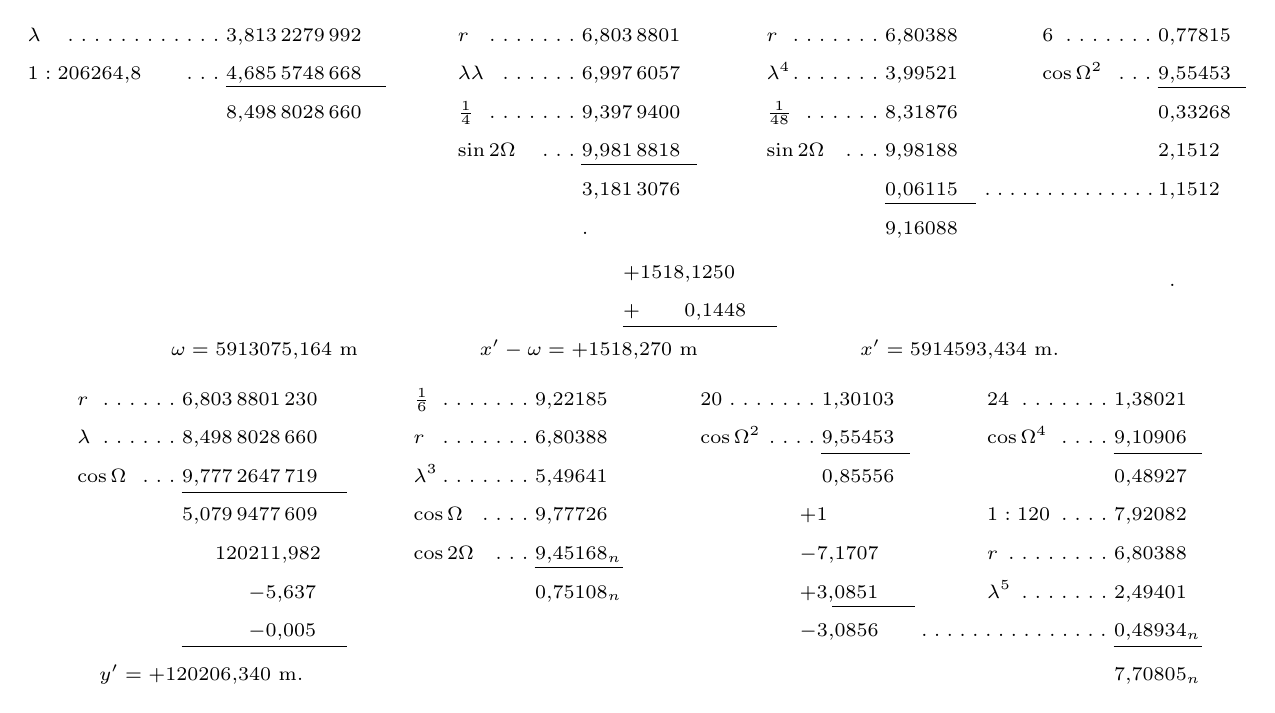
\begin{tikzpicture}[x=.007cm,y=-.007cm,every node/.style={anchor=base west,inner sep=0pt,font=\fontsize{7.5}{9}\selectfont},line width=.3pt]
\node at (0,0) {$\lambda$};
\node at (72,0) {$.$};
\node at (96,0) {$.$};
\node at (120,0) {$.$};
\node at (144,0) {$.$};
\node at (168,0) {$.$};
\node at (192,0) {$.$};
\node at (216,0) {$.$};
\node at (240,0) {$.$};
\node at (264,0) {$.$};
\node at (288,0) {$.$};
\node at (312,0) {$.$};
\node at (336,0) {$.$};
\node at (360,0) {$3{,}813\,2279\,992$};
\node at (0,70) {$1:206264{,}8$};
\node at (288,70) {$.$};
\node at (312,70) {$.$};
\node at (336,70) {$.$};
\node at (360,70) {$4{,}685\,5748\,668$};
\draw (360,82)--(650,82);
\node at (360,140) {$8{,}498\,8028\,660$};
\node at (780,0) {$r$};
\node at (837,0) {$.$};
\node at (861,0) {$.$};
\node at (885,0) {$.$};
\node at (909,0) {$.$};
\node at (933,0) {$.$};
\node at (957,0) {$.$};
\node at (981,0) {$.$};
\node at (1005,0) {$6{,}803\,8801$};
\node at (780,70) {$\lambda\lambda$};
\node at (861,70) {$.$};
\node at (885,70) {$.$};
\node at (909,70) {$.$};
\node at (933,70) {$.$};
\node at (957,70) {$.$};
\node at (981,70) {$.$};
\node at (1005,70) {$6{,}997\,6057$};
\node at (780,140) {$\frac14$};
\node at (837,140) {$.$};
\node at (861,140) {$.$};
\node at (885,140) {$.$};
\node at (909,140) {$.$};
\node at (933,140) {$.$};
\node at (957,140) {$.$};
\node at (981,140) {$.$};
\node at (1005,140) {$9{,}397\,9400$};
\node at (780,210) {$\sin2\Omega$};
\node at (933,210) {$.$};
\node at (957,210) {$.$};
\node at (981,210) {$.$};
\node at (1005,210) {$9{,}981\,8818$};
\draw (1005,224)--(1215,224);
\node at (1005,280) {$3{,}181\,3076$};
\node at (1340,0) {$r$};
\node at (1387,0) {$.$};
\node at (1411,0) {$.$};
\node at (1435,0) {$.$};
\node at (1459,0) {$.$};
\node at (1483,0) {$.$};
\node at (1507,0) {$.$};
\node at (1531,0) {$.$};
\node at (1555,0) {$6{,}80388$};
\node at (1340,70) {$\lambda^4$};
\node at (1387,70) {$.$};
\node at (1411,70) {$.$};
\node at (1435,70) {$.$};
\node at (1459,70) {$.$};
\node at (1483,70) {$.$};
\node at (1507,70) {$.$};
\node at (1531,70) {$.$};
\node at (1555,70) {$3{,}99521$};
\node at (1340,140) {$\frac1{48}$};
\node at (1411,140) {$.$};
\node at (1435,140) {$.$};
\node at (1459,140) {$.$};
\node at (1483,140) {$.$};
\node at (1507,140) {$.$};
\node at (1531,140) {$.$};
\node at (1555,140) {$8{,}31876$};
\node at (1340,210) {$\sin2\Omega$};
\node at (1483,210) {$.$};
\node at (1507,210) {$.$};
\node at (1531,210) {$.$};
\node at (1555,210) {$9{,}98188$};
\node at (1555,280) {$0{,}06115$};
\draw (1555,295)--(1720,295);
\node at (1555,350) {$9{,}16088$};
\node at (1840,0) {$6$};
\node at (1882,0) {$.$};
\node at (1906,0) {$.$};
\node at (1930,0) {$.$};
\node at (1954,0) {$.$};
\node at (1978,0) {$.$};
\node at (2002,0) {$.$};
\node at (2026,0) {$.$};
\node at (2050,0) {$0{,}77815$};
\node at (1840,70) {$\cos\Omega^2$};
\node at (1978,70) {$.$};
\node at (2002,70) {$.$};
\node at (2026,70) {$.$};
\node at (2050,70) {$9{,}55453$};
\draw (2050,84)--(2210,84);
\node at (2050,140) {$0{,}33268$};
\node at (2050,210) {$2{,}1512$};
\node at (2050,280) {$1{,}1512$};
\node at (1735.00,280) {$.$};
\node at (1757.69,280) {$.$};
\node at (1780.38,280) {$.$};
\node at (1803.08,280) {$.$};
\node at (1825.77,280) {$.$};
\node at (1848.46,280) {$.$};
\node at (1871.15,280) {$.$};
\node at (1893.85,280) {$.$};
\node at (1916.54,280) {$.$};
\node at (1939.23,280) {$.$};
\node at (1961.92,280) {$.$};
\node at (1984.62,280) {$.$};
\node at (2007.31,280) {$.$};
\node at (2030.00,280) {$.$};
\node at (1005,350) {$.$};
\node at (2070,445) {$.$};
\node at (1080,430) {$+1518{,}1250$};
\node at (1080,500) {$+\phantom{1518}0{,}1448$};
\draw (1080,518)--(1360,518);
\node at (260,570) {$\omega=5913075{,}164\ \mathrm m$};
\node at (820,570) {$x'-\omega=+1518{,}270\ \mathrm m$};
\node at (1510,570) {$x'=5914593{,}434\ \mathrm m.$};

\node at (90,660) {$r$};
\node at (136,660) {$.$};
\node at (160,660) {$.$};
\node at (184,660) {$.$};
\node at (208,660) {$.$};
\node at (232,660) {$.$};
\node at (256,660) {$.$};
\node at (280,660) {$6{,}803\,8801\,230$};
\node at (90,730) {$\lambda$};
\node at (136,730) {$.$};
\node at (160,730) {$.$};
\node at (184,730) {$.$};
\node at (208,730) {$.$};
\node at (232,730) {$.$};
\node at (256,730) {$.$};
\node at (280,730) {$8{,}498\,8028\,660$};
\node at (90,800) {$\cos\Omega$};
\node at (208,800) {$.$};
\node at (232,800) {$.$};
\node at (256,800) {$.$};
\node at (280,800) {$9{,}777\,2647\,719$};
\draw (280,818)--(580,818);
\node at (280,870) {$5{,}079\,9477\,609$};
\node at (340,940) {$120211{,}982$};
\node at (400,1010) {$-5{,}637$};
\node at (400,1080) {$-0{,}005$};
\draw (280,1098)--(580,1098);
\node at (130,1160) {$y'=+120206{,}340\ \mathrm m.$};
\node at (700,660) {$\frac16$};
\node at (752,660) {$.$};
\node at (776,660) {$.$};
\node at (800,660) {$.$};
\node at (824,660) {$.$};
\node at (848,660) {$.$};
\node at (872,660) {$.$};
\node at (896,660) {$.$};
\node at (920,660) {$9{,}22185$};
\node at (700,730) {$r$};
\node at (752,730) {$.$};
\node at (776,730) {$.$};
\node at (800,730) {$.$};
\node at (824,730) {$.$};
\node at (848,730) {$.$};
\node at (872,730) {$.$};
\node at (896,730) {$.$};
\node at (920,730) {$6{,}80388$};
\node at (700,800) {$\lambda^3$};
\node at (752,800) {$.$};
\node at (776,800) {$.$};
\node at (800,800) {$.$};
\node at (824,800) {$.$};
\node at (848,800) {$.$};
\node at (872,800) {$.$};
\node at (896,800) {$.$};
\node at (920,800) {$5{,}49641$};
\node at (700,870) {$\cos\Omega$};
\node at (824,870) {$.$};
\node at (848,870) {$.$};
\node at (872,870) {$.$};
\node at (896,870) {$.$};
\node at (920,870) {$9{,}77726$};
\node at (700,940) {$\cos2\Omega$};
\node at (848,940) {$.$};
\node at (872,940) {$.$};
\node at (896,940) {$.$};
\node at (920,940) {$9{,}45168_n$};
\draw (920,955)--(1080,955);
\node at (920,1010) {$0{,}75108_n$};
\node at (1220,660) {$20$};
\node at (1272,660) {$.$};
\node at (1296,660) {$.$};
\node at (1320,660) {$.$};
\node at (1344,660) {$.$};
\node at (1368,660) {$.$};
\node at (1392,660) {$.$};
\node at (1416,660) {$.$};
\node at (1440,660) {$1{,}30103$};
\node at (1220,730) {$\cos\Omega^2$};
\node at (1344,730) {$.$};
\node at (1368,730) {$.$};
\node at (1392,730) {$.$};
\node at (1416,730) {$.$};
\node at (1440,730) {$9{,}55453$};
\draw (1440,748)--(1600,748);
\node at (1440,800) {$0{,}85556$};
\node at (1400,870) {$+1$};
\node at (1400,940) {$-7{,}1707$};
\node at (1400,1010) {$+3{,}0851$};
\draw (1460,1025)--(1610,1025);
\node at (1400,1080) {$-3{,}0856$};
\node at (1740,660) {$24$};
\node at (1802,660) {$.$};
\node at (1826,660) {$.$};
\node at (1850,660) {$.$};
\node at (1874,660) {$.$};
\node at (1898,660) {$.$};
\node at (1922,660) {$.$};
\node at (1946,660) {$.$};
\node at (1970,660) {$1{,}38021$};
\node at (1740,730) {$\cos\Omega^4$};
\node at (1874,730) {$.$};
\node at (1898,730) {$.$};
\node at (1922,730) {$.$};
\node at (1946,730) {$.$};
\node at (1970,730) {$9{,}10906$};
\draw (1970,748)--(2130,748);
\node at (1970,800) {$0{,}48927$};
\node at (1740,870) {$1:120$};
\node at (1874,870) {$.$};
\node at (1898,870) {$.$};
\node at (1922,870) {$.$};
\node at (1946,870) {$.$};
\node at (1970,870) {$7{,}92082$};
\node at (1740,940) {$r$};
\node at (1778,940) {$.$};
\node at (1802,940) {$.$};
\node at (1826,940) {$.$};
\node at (1850,940) {$.$};
\node at (1874,940) {$.$};
\node at (1898,940) {$.$};
\node at (1922,940) {$.$};
\node at (1946,940) {$.$};
\node at (1970,940) {$6{,}80388$};
\node at (1740,1010) {$\lambda^5$};
\node at (1802,1010) {$.$};
\node at (1826,1010) {$.$};
\node at (1850,1010) {$.$};
\node at (1874,1010) {$.$};
\node at (1898,1010) {$.$};
\node at (1922,1010) {$.$};
\node at (1946,1010) {$.$};
\node at (1970,1010) {$2{,}49401$};
\node at (1970,1080) {$0{,}48934_n$};
\draw (1970,1098)--(2130,1098);
\node at (1970,1160) {$7{,}70805_n$};
\node at (1620.00,1080) {$.$};
\node at (1643.21,1080) {$.$};
\node at (1666.43,1080) {$.$};
\node at (1689.64,1080) {$.$};
\node at (1712.86,1080) {$.$};
\node at (1736.07,1080) {$.$};
\node at (1759.29,1080) {$.$};
\node at (1782.50,1080) {$.$};
\node at (1805.71,1080) {$.$};
\node at (1828.93,1080) {$.$};
\node at (1852.14,1080) {$.$};
\node at (1875.36,1080) {$.$};
\node at (1898.57,1080) {$.$};
\node at (1921.79,1080) {$.$};
\node at (1945.00,1080) {$.$};
\end{tikzpicture}
\end{center}
\begin{center}\rule{4cm}{.4pt}\end{center}
Concerning Art.~[30], note that \textsc{Gauss}'s logarithmic table (\textsc{von Zach}'s \emph{Monatliche Correspondenz}. Vol.~XXVI. Gotha 1812, pp.~498---528) gives
\[
\mathrm A=\log n,\qquad\mathrm B=\log\left(1+\frac1n\right),\qquad
\mathrm C=\log(1+n),
\]
where $n$ denotes a positive number. $\mathrm A+\mathrm B=\mathrm C$.

Setting $\mathrm C=2\log\sec\psi=\frac{k\pi y}{10^7}$ gives $\mathrm A=2\log\operatorname{tang}\psi$, $\mathrm B=-2\log\sin\psi$. Setting $\mathrm B=2\log\sec\psi=\frac{k\pi y}{10^7}$ gives $\mathrm A=-2\log\operatorname{tang}\psi$, $\mathrm C=-2\log\sin\psi$. This yields the stated values for $\log\frac{\sin iy}{i}=\log\frac{\sin\psi^2}{2\cos\psi}$.
\begin{center}\rule{4cm}{.4pt}\end{center}
\bigskip
The two formulas in [32] are obtained as follows.

Setting $\Phi=90^\circ-p$, we have by 2) and 3), p.~199, when the origin of coordinates corresponds to a fixed point on the principal meridian,
\[
\begin{array}{r@{\qquad}l}
1)&\displaystyle\mathrm f(\xi)=\log\operatorname{hyp}
\left(\operatorname{cotang}\frac p2.\left(\frac{1-e\cos p}{1+e\cos p}\right)^{\frac12e}\right)-K,
\end{array}
\]
\par\endgroup
\vfill\noindent\hfill26\textsuperscript{$\ast$}\hspace*{2cm}
\clearpage
\noindent204\hfill\textsc{Remarks. Conformal Mapping of the Spheroid in the Plane.}\par\medskip
\begingroup\footnotesize
where $K$ is the value of the logarithm at the origin. Hence
\[
\mathrm f(\xi)+i\lambda=\log\operatorname{hyp}\left\{\operatorname{cotang}\frac p2.\left(\frac{1-e\cos p}{1+e\cos p}\right)^{\frac12e}.(\cos\lambda+i\sin\lambda)\right\}-K.
\]
Here $\xi$ is also the length of the meridian arc from the origin to latitude $90^\circ-p$. Like the abscissae, this arc is to be counted positive southward. Thus
\[
\begin{array}{r@{\qquad}l}
2)&\displaystyle\xi=\int\frac{a(1-ee)\,\mathrm dp}{\sqrt{(1-ee\cos p^2)^3}}.
\end{array}
\]
Now set
\[
\begin{array}{r@{\quad}l}
3)&\displaystyle\operatorname{cotang}\frac P2.\left(\frac{1-e\cos P}{1+e\cos P}\right)^{\frac12e}
=\operatorname{cotang}\frac p2.\left(\frac{1-e\cos p}{1+e\cos p}\right)^{\frac12e}.(\cos\lambda+i\sin\lambda),
\end{array}
\]
where, for $\lambda=0$, we have $P=p$, as well as $y=0$ and $x=\xi$. Then, since $\mathrm f(\xi)+i\lambda=\mathrm f(x+iy)$, we have
\[
\begin{array}{r@{\qquad}l}
4)&\displaystyle\mathrm f(x+iy)=\log\operatorname{hyp}\left(\operatorname{cotang}\frac P2.\left(\frac{1-e\cos P}{1+e\cos P}\right)^{\frac12e}\right)-K;
\end{array}
\]
and consequently the equation corresponding to 2)
\[
\begin{array}{r@{\qquad}l}
5)&\displaystyle x+iy=\int\frac{a(1-ee)\,\mathrm dP}{\sqrt{(1-ee\cos P)^3}}
\end{array}
\]
must hold.
\begin{center}\rule{4cm}{.4pt}\end{center}
\bigskip
The developments for articles [1]--[15], [21] and [22] probably date from between 1816 and 1820, while the remaining articles appear to date from the years 1825--1827.
\begin{flushright}\textsc{Krüger.}\end{flushright}
\begin{center}\rule{7cm}{.5pt}\end{center}
\par\endgroup
\clearpage
% The source opening leaf [205] has no printed folio or running header.
\vspace*{1.3cm}
\begin{center}
{\Large\bfseries CORRESPONDENCE.}\par
\vspace{1.7cm}
{\large\bfseries [On the Formulas for the Hanoverian Land Survey.]}\par
\bigskip
\textsc{Gauss} to \textsc{Schumacher}.\quad Göttingen, 18~April 1830.
\end{center}
\medskip
.\ .\ .\ .\ .\ .\ In your survey, if you intend to restrict yourself to one of the two methods discussed in my earlier letter, it seems to me most appropriate for you to calculate your results for the positions of the individual points in coordinate form. From these coordinates you can then calculate longitudes and latitudes for all the points for which you find this necessary. This procedure requires only a few compact auxiliary tables. Indeed, all the tables then needed can fit on one octavo page. The distinctive features of the method are then also very easy to learn. The material will fall into two chapters.

I. Modifications that the calculation of the coordinates must undergo because the surface of the Earth is not planar. This requires a short treatise, and the calculation itself requires a small auxiliary table.

II. Method for calculating from the given coordinates of a point 1) its longitude, 2) its latitude, 3) the direction of its meridian in the coordinate system.

This will require a second treatise and several small auxiliary tables. I shall begin with this chapter today.

The distance of a point from the equator, measured in fractions $\frac1{90}$, $\frac1{90.60}$, $\frac1{90.60.60}$ of the entire terrestrial quadrant instead of in toises or some other similar unit, I denote by $\psi$, and the latitude of the same point by $\varphi$. One problem, then, is to find $\varphi$ from $\psi$.
\clearpage
\noindent206\hfill\textsc{Correspondence.}\hfill\mbox{}\par\medskip
I do this with a table that, with $\psi$ as its argument, gives $\varphi-\psi$ directly. I have calculated this table using \textsc{Schmidt}'s latest flattening $\frac1{297{,}732}$ from $51^\circ$ to $56^\circ$, and I send it to you here.
\begin{center}
\renewcommand{\arraystretch}{1.07}
\begin{tabular}[t]{|r@{\;}r|r@{\;}r|}
\hline
\multicolumn{2}{|c|}{$\psi$}&\multicolumn{2}{c|}{$\varphi-\psi$}\\\hline\hline
$51^\circ$&$0'$&$8'$&$28''{,}78$\\\hline
&$10$&&$28{,}14$\\
&$20$&&$27{,}47$\\
&$30$&&$26{,}79$\\
&$40$&&$26{,}10$\\
&$50$&&$25{,}38$\\
$52$&$0$&$8$&$24{,}65$\\\hline
&$10$&&$23{,}90$\\
&$20$&&$23{,}13$\\
&$30$&&$22{,}35$\\
&$40$&&$21{,}55$\\
&$50$&&$20{,}73$\\
$53$&$0$&$8$&$19{,}90$\\\hline
&$10$&&$19{,}05$\\
&$20$&&$18{,}18$\\
&$30$&&$17{,}30$\\
&$40$&&$16{,}40$\\
&$50$&&$15{,}48$\\
$54$&$0$&$8$&$14{,}54$
\end{tabular}
\hspace{2cm}
\begin{tabular}[t]{|r@{\;}r|r@{\;}r|}
\hline
\multicolumn{2}{|c|}{$\psi$}&\multicolumn{2}{c|}{$\varphi-\psi$}\\\hline\hline
$54^\circ$&$0'$&$8'$&$14''{,}54$\\\hline
&$10$&&$13{,}59$\\
&$20$&&$12{,}63$\\
&$30$&&$11{,}64$\\
&$40$&&$10{,}64$\\
&$50$&&$9{,}62$\\
$55$&$0$&$8$&$8{,}59$\\\hline
&$10$&&$7{,}54$\\
&$20$&&$6{,}47$\\
&$30$&&$5{,}39$\\
&$40$&&$4{,}29$\\
&$50$&&$3{,}17$\\
$56$&$0$&$8$&$2{,}04$
\end{tabular}
\end{center}
If you wish to extend this table or calculate it to more decimal places, the following formula serves that purpose.
\[
\begin{aligned}
\varphi=\psi&+520''{,}4633364\sin2\psi\\
&+0{,}7660757\sin4\psi\\
&+0{,}0015444\sin6\psi\\
&+0{,}0000035\sin8\psi.
\end{aligned}
\]
No instructions are needed for finding $\psi$ for any point on the principal meridian from its $x$ and the value of $\psi$ corresponding to the origin, $\psi^\circ$, since this is a simple rule-of-three calculation.
\clearpage
\noindent{\small\textsc{On the Formulas for the Hanoverian Land Survey.}}\hfill207\par\medskip
Naturally this preliminary calculation is more or less expeditious depending on the choice of the unit of length. For this reason, and for others, I have chosen the 10\,000\,000th part of the terrestrial quadrant as my unit of length. For brevity I call it a metre, though it differs from the legal metre. With \textsc{Schmidt}'s dimensions my metre is $443^{\mathrm{lin}}{,}29849$. Therefore setting
\[
\psi=\psi^\circ-0''{,}0324.x\ [=\psi^\circ-0'{,}00054.x]
\]
is enough. If you choose toises, the equation
\[
\psi=\psi^\circ-1^\circ.\frac{x}{57008{,}551}
\]
must be written.

You can also easily find $\psi^\circ$ indirectly from the auxiliary table above if $\varphi^\circ$ is given. For Göttingen I set
\[
\psi^\circ=51^\circ23'20''{,}6082,
\]
to which $\varphi^\circ=51^\circ31'47''{,}85$ corresponds.

If, for example, $x=-115163{,}725$ toises, we obtain
\[
\begin{array}{r@{\quad}r@{\;}r@{\;}r}
\psi=&51^\circ&23'&20''{,}6082\\
+&2&1&12{,}4074\\\cline{2-4}
=&53&24&33{,}02
\end{array}
\]
From this the table gives
\[
\varphi=53^\circ32'50''{,}80.
\]
This is the latitude of your meridian circle when it is derived from the latitude of mine using \textsc{Schmidt}'s dimensions for the Earth.

This differs from my astronomical determination by $5''{,}53$. These $5''{,}53$ are the sum of the irregularities in the figure of the Earth at Göttingen and Altona (more precisely, the algebraic difference). The latitude $53^\circ32'45''{,}27$ would correspond to $\psi=53^\circ24'27''{,}48$. So if one wished to divide that difference equally, one could also set
\[
\begin{array}{r@{\quad}r@{\;}r@{\;}r}
\text{for Göttingen: }\psi=&51^\circ&23'&17''{,}84\\
\text{for Altona: }\psi=&53&24&30{,}25.
\end{array}
\]
\clearpage
\noindent208\hfill\textsc{Correspondence.}\hfill\mbox{}\par\medskip
As for the main problem, I denote the given coordinates [by] $x$, $y$. I denote the latitude (calculated according to the rule above) of the point whose coordinates are $x$ and $0$ by $\varphi$, the longitude sought by $\lambda$ (reckoned from the principal meridian), the latitude sought by $\Phi$, and the angle that the meridian of the place makes with the line of constant $y$ (the convergence of the meridians) by $c$.

These\raisebox{.65ex}{.} three quantities can then be expressed by series of the following form
\[
\begin{aligned}
\llap{\text{\raisebox{.45ex}{.}\hspace{1em}}}\lambda&=\alpha y-\beta y^3+\gamma y^5-\text{etc.}\\
\Phi&=\varphi-\alpha'yy+\beta'y^4-\gamma'y^6+\text{etc.}\\
c&=\alpha''y-\beta''y^3+\gamma''y^5-\text{etc.},
\end{aligned}
\]
where the coefficients $\alpha$, $\alpha'$, $\alpha''$, $\beta$, etc. depend on $\varphi$. In the cases to which I restrict the use of the coordinate method, however, one never needs to go beyond $y^4$. On this assumption I find it more convenient to modify the form of the series slightly. Namely, I set $\alpha y=l$ and then write
\[
\begin{aligned}
\lambda&=\frac lA\\
\Phi&=\varphi-\frac{\alpha'yy}{B}\\
c&=\frac{\alpha''y}{C},
\end{aligned}
\]
where $A$, $B$, $C$ will be only very slightly greater than $1$. The Briggsian logarithms can now simply be set equal to
\[
\begin{aligned}
\log A&=Dll\\
\log B&=Ell\\
\log C&=Fll,
\end{aligned}
\]
where $D$, $E$, $F$ are functions of $\varphi$. For example, $D=\frac{\beta k}{\alpha^3}$ if $k$ is the modulus of the Briggsian logarithms, or, if $\log A$ is to be expressed directly in units of the seventh decimal place, $D=\frac{10^7.\beta k}{\alpha^3}$ (as it is to be understood in my table copied below).

Thus we need only a second auxiliary table, which could be arranged to give, with $\varphi$ as the argument, the logarithms of $\alpha$, $\alpha'$, $\alpha''$, $D$, $E$ and $F$. Here too, however, it is more convenient to make a slight modi-\par
\clearpage
\noindent{\small\textsc{On the Formulas for the Hanoverian Land Survey.}}\hfill209\par\medskip
\noindent fication. Namely, setting the eccentricity $=e$ and the radius of the Earth's equator $=a$, we have
\[
\begin{aligned}
\alpha&=\frac{\sqrt{(1-ee\sin\varphi^2)}}{a\cos\varphi}.206265\\
\alpha'&=\frac{(1-ee\sin\varphi^2)^2.\operatorname{tang}\varphi}{2aa(1-ee)}.206265\\
\alpha''&=\frac{\sqrt{(1-ee\sin\varphi^2)}}a.\operatorname{tang}\varphi.206265.
\end{aligned}
\]
I therefore write
\[
\begin{aligned}
\frac{206265.\sqrt{(1-ee\sin\varphi^2)}}a&=G\\
\frac{206265.(1-ee\sin\varphi^2)^2}{2aa(1-ee)}&=H,
\end{aligned}
\]
and include in my table, in place of the logarithms of $\alpha$, $\alpha'$, $\alpha''$, those of $G$ and $H$. In this way I save one column, and I gain the advantage that the values of these logarithms change very slowly. I therefore need to advance the argument $\varphi$ in the table only from one $10$-minute mark to the next $10$-minute mark, whereas a table for $\log\alpha$, etc. themselves would have to be intolerably large to be convenient to use. The entire calculation therefore rests on the formulas[*)]
\[
\begin{array}{r@{\qquad}l}
1)&\displaystyle l=\frac{Gy}{\cos\varphi},\\[3pt]
2)&\log A=Dll\\[3pt]
3)&\log B=Ell\\[3pt]
4)&\log C=Fll;\\[3pt]
5)&\displaystyle\lambda=\frac lA\\[3pt]
6)&\displaystyle\Phi=\varphi\mathbin{\overset{\raisebox{.15ex}{\scriptsize.}}{-}}\frac{Hyy\operatorname{tang}\varphi}{B}\\[3pt]
7)&\displaystyle c=\frac{Gy\operatorname{tang}\varphi}{C}.
\end{array}
\]
I have calculated this table from $\varphi=51^\circ$ to $\varphi=55^\circ$ and send it to you. Note, however, that if you choose another unit of length, toises for example, your $\log G$ must exceed mine by the logarithm of the ratio $\left(\text{by }\log\frac{864}{443{,}29849}\right)$, and your $\log H$ by twice that amount. Should you ever wish to extend the table any
\par\medskip\noindent\rule{4cm}{.4pt}\par
{\footnotesize [*) Cf. Art.~3, p.~148.]\par}
\vfill\noindent{\footnotesize IX.}\hfill27\hfill\mbox{}\par
\clearpage
\noindent210\hfill\textsc{Correspondence.}\hfill\mbox{}\par\medskip
\noindent further, I shall gladly send you the formulas for $D$, $E$ and $F$ (those for $G$ and $H$ have already been given above).

To illustrate, I give the calculation of an example twice, first with \textsc{Delambre}'s expansiveness, and then in the form in which I usually write the calculation myself, leaving out everything superfluous.\ .\ .\ .\ .\ .\ .\ .\ .\ .
\begin{center}
Second auxiliary table.\par\medskip
\begingroup\small\setlength{\tabcolsep}{5pt}\renewcommand{\arraystretch}{1.08}
\begin{tabular}{|r@{\;}r|r|r|r|r|r|}
\hline
\multicolumn{2}{|c|}{$\varphi$}&$\log G$&$\log H$&$\log D$&$\log E$&$\log F$\\\hline\hline
&&$-10$&$-10$&$-10$&$-10$&$-10$\\
$51^\circ$&$0'$&$8{,}508\,9341$&$1{,}403\,5727$&$5{,}43626$&$5{,}50708$&$5{,}53135$\\
&$10$&$299$&$561$&$703$&$643$&$36$\\
&$20$&$258$&$395$&$779$&$578$&$36$\\
&$30$&$216$&$229$&$855$&$513$&$37$\\
&$40$&$175$&$1{,}403\,5063$&$5{,}43931$&$448$&$38$\\
&$50$&$133$&$1{,}403\,4898$&$5{,}44006$&$383$&$38$\\\hline
$52$&$0$&$8{,}508\,9092$&$1{,}403\,4733$&$5{,}44082$&$5{,}50317$&$5{,}53139$\\
&$10$&$051$&$568$&$157$&$252$&$40$\\
&$20$&$8{,}508\,9010$&$403$&$231$&$187$&$40$\\
&$30$&$8{,}508\,8969$&$239$&$306$&$122$&$41$\\
&$40$&$928$&$1{,}403\,4074$&$380$&$5{,}50057$&$41$\\
&$50$&$887$&$1{,}403\,3910$&$454$&$5{,}49992$&$42$\\\hline
$53$&$0$&$8{,}508\,8846$&$1{,}403\,3747$&$5{,}44528$&$5{,}49927$&$5{,}53143$\\
&$10$&$805$&$583$&$602$&$862$&$43$\\
&$20$&$764$&$420$&$675$&$797$&$44$\\
&$30$&$723$&$257$&$748$&$732$&$44$\\
&$40$&$683$&$1{,}403\,3095$&$821$&$667$&$45$\\
&$50$&$642$&$1{,}403\,2932$&$894$&$602$&$46$\\\hline
$54$&$0$&$8{,}508\,8602$&$1{,}403\,2770$&$5{,}44966$&$5{,}49537$&$5{,}53146$\\
&$10$&$561$&$609$&$5{,}45038$&$472$&$47$\\
&$20$&$521$&$447$&$110$&$407$&$47$\\
&$30$&$481$&$286$&$182$&$342$&$48$\\
&$40$&$440$&$1{,}403\,2125$&$253$&$278$&$48$\\
&$50$&$400$&$1{,}403\,1965$&$324$&$213$&$49$\\\hline
$55$&$0$&$8{,}508\,8360$&$1{,}403\,1805$&$5{,}45395$&$5{,}49148$&$5{,}53149$\\
\end{tabular}\par\endgroup
\end{center}
\underline{Note}. In coordinates I communicated earlier, the unit is $\frac1{10000000}$ of the terrestrial quadrant according to \textsc{Walbeck}'s dimensions. To convert them into coordinates based on the unit $\frac1{10000000}$ of the terrestrial quadrant according to \textsc{Schmidt}'s latest dimensions, they must first be multiplied by $\frac{57009738}{57008551}$ or by $1+\frac1{47282}$.
\clearpage
\noindent{\small\textsc{On the Formulas for the Hanoverian Land Survey.}}\hfill211\par\medskip
\begin{center}
Detailed sample calculation for\\Neuwerk.\par\medskip
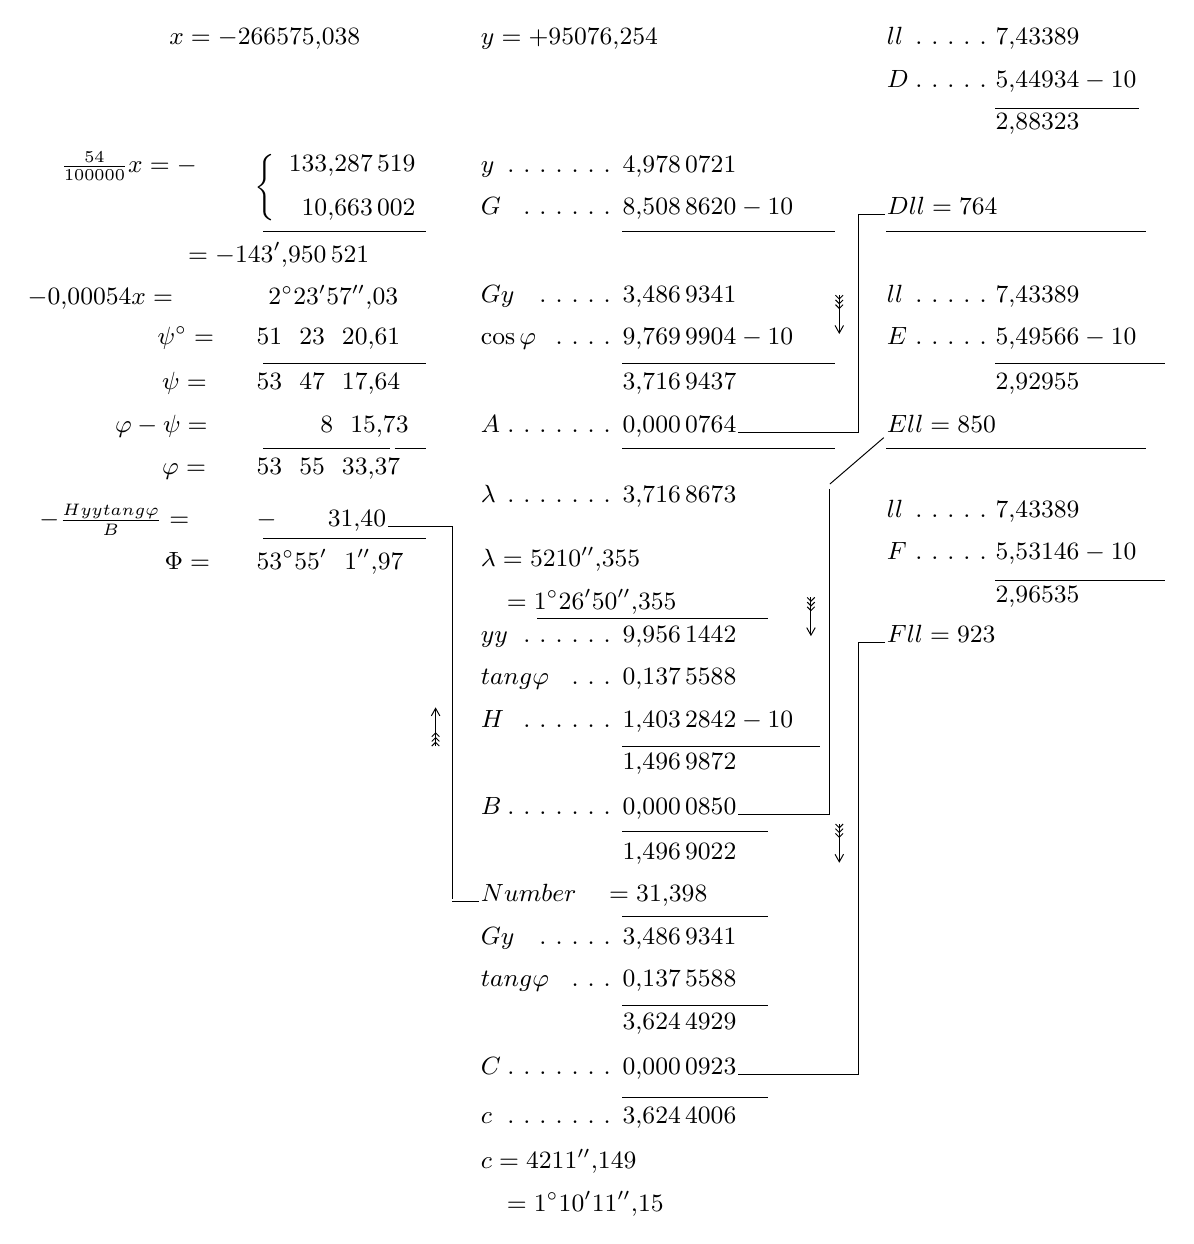
\begin{tikzpicture}[x=.006cm,y=-.006cm,every node/.style={anchor=base west,inner sep=0pt,font=\fontsize{8.8}{10}\selectfont},line width=.35pt]
\node at (280,60) {$x=-266575{,}038$};
\node at (940,60) {$y=+95076{,}254$};
\node at (50,330) {$\frac{54}{100000}x=-$};
\node at (460,375) {$\left\{\begin{array}{r}133{,}287\,519\\[5pt]10{,}663\,002\end{array}\right.$};
\draw (480,455) -- (825,455);
\node at (320,520) {$=-143'{,}950\,521$};
\node at (-20,610) {$-0{,}00054x=$};
\node at (490,610) {$2^\circ23'57''{,}03$};
\node at (255,695) {$\psi^\circ=$};
\node at (465,695) {$51\ \ 23\ \ 20{,}61$};
\draw (480,735) -- (825,735);
\node at (265,790) {$\psi=$};
\node at (465,790) {$53\ \ 47\ \ 17{,}64$};
\node at (165,880) {$\varphi-\psi=$};
\node at (600,880) {$8\ \ 15{,}73$};
\draw (480,915) -- (748,915);
\draw (758,915) -- (825,915);
\node at (265,970) {$\varphi=$};
\node at (465,970) {$53\ \ 55\ \ 33{,}37$};
\node at (5,1080) {$-\frac{Hyy\operatorname{tang}\varphi}{B}=$};
\node (PhiCorrection) at (465,1080) {$-\qquad31{,}40$};
\draw (480,1105) -- (825,1105);
\node at (270,1170) {$\Phi=$};
\node at (465,1170) {$53^\circ55'\ \ 1''{,}97$};
\node at (940,330) {$y$};
\node at (996,330) {$.$};
\node at (1030,330) {$.$};
\node at (1064,330) {$.$};
\node at (1098,330) {$.$};
\node at (1132,330) {$.$};
\node at (1166,330) {$.$};
\node at (1200,330) {$.$};
\node at (1240,330) {$4{,}978\,0721$};
\node at (940,420) {$G$};
\node at (1030,420) {$.$};
\node at (1064,420) {$.$};
\node at (1098,420) {$.$};
\node at (1132,420) {$.$};
\node at (1166,420) {$.$};
\node at (1200,420) {$.$};
\node at (1240,420) {$8{,}508\,8620-10$};
\node at (940,605) {$Gy$};
\node at (1064,605) {$.$};
\node at (1098,605) {$.$};
\node at (1132,605) {$.$};
\node at (1166,605) {$.$};
\node at (1200,605) {$.$};
\node at (1240,605) {$3{,}486\,9341$};
\node at (940,695) {$\cos\varphi$};
\node at (1098,695) {$.$};
\node at (1132,695) {$.$};
\node at (1166,695) {$.$};
\node at (1200,695) {$.$};
\node at (1240,695) {$9{,}769\,9904-10$};
\node at (940,880) {$A$};
\node at (996,880) {$.$};
\node at (1030,880) {$.$};
\node at (1064,880) {$.$};
\node at (1098,880) {$.$};
\node at (1132,880) {$.$};
\node at (1166,880) {$.$};
\node at (1200,880) {$.$};
\node (Aval) at (1240,880) {$0{,}000\,0764$};
\node at (940,1030) {$\lambda$};
\node at (996,1030) {$.$};
\node at (1030,1030) {$.$};
\node at (1064,1030) {$.$};
\node at (1098,1030) {$.$};
\node at (1132,1030) {$.$};
\node at (1166,1030) {$.$};
\node at (1200,1030) {$.$};
\node at (1240,1030) {$3{,}716\,8673$};
\node at (940,1325) {$yy$};
\node at (1030,1325) {$.$};
\node at (1064,1325) {$.$};
\node at (1098,1325) {$.$};
\node at (1132,1325) {$.$};
\node at (1166,1325) {$.$};
\node at (1200,1325) {$.$};
\node at (1240,1325) {$9{,}956\,1442$};
\node at (940,1415) {$\operatorname{tang}\varphi$};
\node at (1132,1415) {$.$};
\node at (1166,1415) {$.$};
\node at (1200,1415) {$.$};
\node at (1240,1415) {$0{,}137\,5588$};
\node at (940,1505) {$H$};
\node at (1030,1505) {$.$};
\node at (1064,1505) {$.$};
\node at (1098,1505) {$.$};
\node at (1132,1505) {$.$};
\node at (1166,1505) {$.$};
\node at (1200,1505) {$.$};
\node at (1240,1505) {$1{,}403\,2842-10$};
\node at (940,1690) {$B$};
\node at (996,1690) {$.$};
\node at (1030,1690) {$.$};
\node at (1064,1690) {$.$};
\node at (1098,1690) {$.$};
\node at (1132,1690) {$.$};
\node at (1166,1690) {$.$};
\node at (1200,1690) {$.$};
\node (Bval) at (1240,1690) {$0{,}000\,0850$};
\node at (940,1965) {$Gy$};
\node at (1064,1965) {$.$};
\node at (1098,1965) {$.$};
\node at (1132,1965) {$.$};
\node at (1166,1965) {$.$};
\node at (1200,1965) {$.$};
\node at (1240,1965) {$3{,}486\,9341$};
\node at (940,2055) {$\operatorname{tang}\varphi$};
\node at (1132,2055) {$.$};
\node at (1166,2055) {$.$};
\node at (1200,2055) {$.$};
\node at (1240,2055) {$0{,}137\,5588$};
\node at (940,2240) {$C$};
\node at (996,2240) {$.$};
\node at (1030,2240) {$.$};
\node at (1064,2240) {$.$};
\node at (1098,2240) {$.$};
\node at (1132,2240) {$.$};
\node at (1166,2240) {$.$};
\node at (1200,2240) {$.$};
\node (Cval) at (1240,2240) {$0{,}000\,0923$};
\node at (940,2345) {$c$};
\node at (996,2345) {$.$};
\node at (1030,2345) {$.$};
\node at (1064,2345) {$.$};
\node at (1098,2345) {$.$};
\node at (1132,2345) {$.$};
\node at (1166,2345) {$.$};
\node at (1200,2345) {$.$};
\node at (1240,2345) {$3{,}624\,4006$};
\node at (1240,790) {$3{,}716\,9437$};
\node at (1240,1595) {$1{,}496\,9872$};
\node at (1240,1785) {$1{,}496\,9022$};
\node at (1240,2145) {$3{,}624\,4929$};
\draw (1240,455) -- (1690,455);
\draw (1240,735) -- (1690,735);
\draw (1240,915) -- (1690,915);
\draw (1060,1275) -- (1550,1275);
\draw (1240,1545) -- (1660,1545);
\draw (1240,1725) -- (1550,1725);
\draw (1240,1905) -- (1550,1905);
\draw (1240,2095) -- (1550,2095);
\draw (1240,2290) -- (1550,2290);
\node at (940,1165) {$\lambda=5210''{,}355$};
\node at (995,1255) {$=1^\circ26'50''{,}355$};
\node (Zahl) at (940,1875) {$\text{Number}\quad=31{,}398$};
\node at (940,2440) {$c=4211''{,}149$};
\node at (995,2530) {$=1^\circ10'11''{,}15$};
\node at (1800,60) {$ll$};
\node at (1860,60) {$.$};
\node at (1894,60) {$.$};
\node at (1928,60) {$.$};
\node at (1962,60) {$.$};
\node at (1996,60) {$.$};
\node at (2030,60) {$7{,}43389$};
\node at (1800,150) {$D$};
\node at (1860,150) {$.$};
\node at (1894,150) {$.$};
\node at (1928,150) {$.$};
\node at (1962,150) {$.$};
\node at (1996,150) {$.$};
\node at (2030,150) {$5{,}44934-10$};
\node at (1800,605) {$ll$};
\node at (1860,605) {$.$};
\node at (1894,605) {$.$};
\node at (1928,605) {$.$};
\node at (1962,605) {$.$};
\node at (1996,605) {$.$};
\node at (2030,605) {$7{,}43389$};
\node at (1800,695) {$E$};
\node at (1860,695) {$.$};
\node at (1894,695) {$.$};
\node at (1928,695) {$.$};
\node at (1962,695) {$.$};
\node at (1996,695) {$.$};
\node at (2030,695) {$5{,}49566-10$};
\node at (1800,1060) {$ll$};
\node at (1860,1060) {$.$};
\node at (1894,1060) {$.$};
\node at (1928,1060) {$.$};
\node at (1962,1060) {$.$};
\node at (1996,1060) {$.$};
\node at (2030,1060) {$7{,}43389$};
\node at (1800,1150) {$F$};
\node at (1860,1150) {$.$};
\node at (1894,1150) {$.$};
\node at (1928,1150) {$.$};
\node at (1962,1150) {$.$};
\node at (1996,1150) {$.$};
\node at (2030,1150) {$5{,}53146-10$};
\node at (2030,240) {$2{,}88323$};
\node at (2030,790) {$2{,}92955$};
\node at (2030,1240) {$2{,}96535$};
\node (Dll) at (1800,420) {$Dll=764$};
\node (Ell) at (1800,880) {$Ell=850$};
\node (Fll) at (1800,1325) {$Fll=923$};
\draw (2030,195) -- (2335,195);
\draw (1800,455) -- (2350,455);
\draw (2030,735) -- (2390,735);
\draw (1800,915) -- (2350,915);
\draw (2030,1195) -- (2390,1195);
\draw ([xshift=-.5pt]Dll.base west) -- (1740,420) -- (1740,880) -- ([xshift=.5pt]Aval.base east);
\draw ([xshift=-1pt,yshift=-2pt]Ell.base west) -- (1680,990);
\draw (1680,1000) -- (1680,1690) -- ([xshift=.5pt]Bval.base east);
\draw ([xshift=-.5pt]Fll.base west) -- (1740,1325) -- (1740,2240) -- ([xshift=.5pt]Cval.base east);
\draw ([xshift=.5pt]PhiCorrection.base east) -- (880,1080) -- (880,1868);
\draw (880,1875) -- ([xshift=-.5pt]Zahl.base west);
\draw (1700,590) -- (1700,670);
\draw (1691,654) -- (1700,670) -- (1709,654);
\draw (1692,590) -- (1700,598) -- (1708,590);
\draw (1692,600) -- (1700,608) -- (1708,600);
\draw (1692,610) -- (1700,618) -- (1708,610);
\draw (1640,1230) -- (1640,1310);
\draw (1631,1294) -- (1640,1310) -- (1649,1294);
\draw (1632,1230) -- (1640,1238) -- (1648,1230);
\draw (1632,1240) -- (1640,1248) -- (1648,1240);
\draw (1632,1250) -- (1640,1258) -- (1648,1250);
\draw (1700,1710) -- (1700,1790);
\draw (1691,1774) -- (1700,1790) -- (1709,1774);
\draw (1692,1710) -- (1700,1718) -- (1708,1710);
\draw (1692,1720) -- (1700,1728) -- (1708,1720);
\draw (1692,1730) -- (1700,1738) -- (1708,1730);
\draw (845,1545) -- (845,1465);
\draw (836,1481) -- (845,1465) -- (854,1481);
\draw (837,1545) -- (845,1537) -- (853,1545);
\draw (837,1535) -- (845,1527) -- (853,1535);
\draw (837,1525) -- (845,1517) -- (853,1525);
\end{tikzpicture}
\end{center}
\vfill\hfill$27^*$\hspace*{2cm}\par
\endgroup
